% standalone document border convention: {left bottom right top}
\documentclass[varwidth=400pt,border={0pt, -2pt, 1pt, -10pt}]{standalone}
\usepackage[force]{feynmp-auto}		    
\usepackage{amsmath}
\usepackage{graphicx}
\usepackage{simpler-wick}

\begin{document}
\begin{flalign*}
	\chi_{1,2} \hspace*{0.5ex}&=\hspace*{0.5ex}
	\xi\hspace*{0.5ex}
	\langle \wick[offset=3ex]{\c2 {\bar{\psi}_2} \c1 \psi_2 \c1 {\bar{\psi}_1} \c2 \psi_1} \rangle_0
	\hspace*{0.5ex}-\xi\hspace*{0.5ex}
	V_{34} \langle \wick[offset=3ex]{
		 \c2 {\bar{\psi}_2} \c1 {\psi_2}
		 \c3 {\bar{\psi}_3} \c1 {\bar{\psi}_4}
		 \c2 {\psi_4} \c1 {\psi_3}
		 \c1 {\bar{\psi}_1} \c3 {\psi_1}
	} \rangle_0
	\hspace*{0.5ex}-\xi\hspace*{0.5ex}
	V_{34} \langle \wick[offset=3ex]{
		\c2 {\bar{\psi}_2} \c1 {\psi_2}
		\c1 {\bar{\psi}_3} \c3 {\bar{\psi}_4}
		\c2 {\psi_4} \c1 {\psi_3}
		\c1 {\bar{\psi}_1} \c3 {\psi_1}
	} \rangle_0 \hspace*{0.5ex}+\hspace*{0.5ex} \cdots \\[1ex]
	&=\hspace*{0.5ex} \xi g_{12} g_{21}
	\hspace*{0.5ex}+\hspace*{0.5ex}
	(-1) V_{34} g_{13} g_{31} g_{24} g_{42}
	\hspace*{0.5ex}+\hspace*{0.5ex}
	(-1)\xi V_{34} g_{13} g_{32} g_{24} g_{41}
	\hspace*{0.5ex}+\hspace*{0.5ex} \cdots \\
	&= \raisebox{-0.15ex}{
	\scalebox{0.75}{$
			\begin{gathered}
				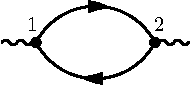
\includegraphics{susceptibility/chi0.pdf}
			\end{gathered}
		$}
	}
	+
	\raisebox{-0.15ex}{
	\scalebox{0.75}{$
			\begin{gathered}
				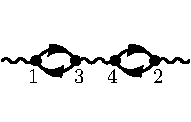
\includegraphics{susceptibility/chi1d.pdf}
			\end{gathered}
		$}
	}
	+
	\raisebox{-0.15ex}{
	\scalebox{0.75}{$
			\begin{gathered}
				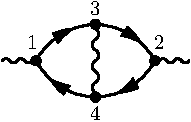
\includegraphics{susceptibility/chi1a.pdf}
			\end{gathered}
		$}
	}
	+ \cdots
\end{flalign*}
\end{document}
